\chapter{Characterization of Heat Transport in Nanometer Scale Systems}

Work presented in this chapter is adapted from the following papers:

\begin{itemize}
\item Hannah, D. C.; Dunn, N. J.; Ithurria, S.; Talapin, D. V.; Chen, L. X.; Pelton, M.; Schatz, G. C.; Schaller, R. D. \emph{Phys. Rev. Lett.} \textbf{2011}, 107, 177403

\item Hannah, D.C.; Gezelter, J.D.; Schaller, R.D.; Schatz, G.C. \emph{ACS Nano} \textbf{2015}, 9, 6278
\end{itemize}
\section{Introduction}

Colloidal semiconductor nanocrystal (NC) quantum dots offer size-tunable band gaps, solution processing, and controllable surface functionality that can impact technologies ranging from lighting \cite{doi:10.1021/nl9002969} and biolabels \cite{doi:10.1146/annurev.bioeng.7.060804.100432} to photovoltaics \cite{Huynh29032002} and thermoelectrics \cite{Hsu06022004, Talapin07102005}.  While much of the materials community focuses on new compositions as well as determination of NC optical properties and incorporation into devices, thermal management, which is crucial to each of the highlighted technologies, will become an increasingly important factor for the use of these thermodynamically compromised materials. Measurement and manipulation of thermal outflow rates in nanoscale semiconductors at present, however, represents a challenge. Comprehensive understanding of the electron-hole pair (“exciton”) dynamics, electronic structure, and thermal properties of such designer materials in aggregate is vital to their successful application.  In this Chapter, we detail an optical signature of phonon outflow from matrix-embedded semiconductor nanocrystals via observation of transient phonon-assisted radiative recombination from the lowest-energy exciton fine structure state (the "dark" exciton state), for which transitions are ordinarily dipole-forbidden. We also utilize a recently-developed MD method to simulate thermal transport at a realistic, chemically passsivated semiconductor/ligand/solvent interface and determine the role played by the ligand layer as well as the crystal structure of the underlying semiconductor in mediating thermal transport rates at this interface.

\subsection{Experimental Challenges}

From a fundamental point of view, the small size of NCs challenges predictions and measurements of thermal transport. While NC radii generally range in size from 1 to 40 nm, phonon mean free paths are typically hundreds of nanometers. Such discrepancy in sizes yields highly diffusive scattering, wherein phonons scatter in all directions upon interaction with a NC interface \cite{chen2000particularities}. Small NC sizes also present experimental challenges.  Technique-specific sample length and size requirements that greatly exceed NC diameters rule out contact-based measurements including hot-wire probes and the $3\omega$ method \cite{chen2000particularities, PhysRevLett.95.065502}. Noncontact probes such as transient absorption permit studies of phonon outflow from metallic nanoparticles via the thermal-broadening of plasmon resonances, but such measurements are not applicable to semiconductor NCs \cite{pelton2009damping,doi:10.1021/jp020581+,pelton2009damping}. Transient thermoreflectance (TTR) uses an optical pump to heat a reflective surface and a time-delayed probe to track temperature induced changes to the reflectivity of the surface \cite{paddock1986transient}. Along with fits to an appropriate thermal transport model, this method is capable of optically measuring thermal conductivity as well as interfacial thermal conductance, and has been successfully applied to densely packed NC films \cite{ong2013surface}. However, such measurements probe surface areas containing tens of thousands of NCs and inherently relay only averaged information about thermal transport. \par

Isolated particles (either suspended as a colloid or in a matrix) can provide information about particle-level thermal transport but do not provide a reflective surface for TTR to be carried out. Colloidal semiconductor materials that present a continuous density of states (DOS), such as one-dimensional quantum confined rods, permit the measurement of thermally populated electronic states \cite{achermann2006effect}; however zero-dimensional NCs exhibit a discrete DOS that prevents utilization of this approach. Examinations of intraband electronic relaxation \cite{PhysRevB.60.R2181,PhysRevLett.80.4028} and coherent phonons \cite{1464-4258-10-6-064004,PhysRevLett.79.5102,PhysRevB.77.235321} in semiconductor NCs suggest that excess carrier energy produces phonons on an ultrafast time scale, but the fate of these phonons remains elusive. Even in cases where coherent phonons are observed, the damping of coherent oscillations likely reflects dephasing in the NC ensemble owing to size polydispersity (each nanocrystal has a slightly different vibrational frequency) rather than actual changes in phonon population.

\subsection{Theoretical Challenges}

Chen and co-workers, among others, note fundamental difficulties associated with applying current heat conduction theories to structures in this size regime \cite{chen2000particularities}. As described in the introduction to this thesis, the extent to which approximations for the phonon distribution function and transmission coefficients apply to the case of chemically passivated interfaces is unclear. While simple, the acoustic mismatch model (AMM) assumes specular reflection/transmission of interfacial phonons - likely a poor assumption for rough interfaces \cite{chen2000particularities} - and at any rate, the acoustic properties of the passivating monolayer are not well characterized or understood for most common materials. The diffuse mismatch model (DMM) is perhaps somewhat more intuitively appealing for an interface displaying at least one highly disordered component. However, it assumes phonon scattering is completely diffuse, i.e. that phonons lose all "memory" of their trajectory upon scattering. This results in transmission probability lacking any dependence on phonon wavevector, which may be a poor approximation for the crystalline side of the interface. Indeed, DMM-based predictions of interfacial thermal conductance often significantly over- or underestimate interfacial thermal conductance at non-cryogenic temperatures \cite{yang2015thermal, duda2009extension}, depending on the materials present. \par

While extensions of the DMM to account for higher temperatures \cite{duda2009extension}, interfacial disorder \cite{beechem2007role}, and inelastic scattering \cite{hopkins2007effects} have improved the accuracy of the model, problems persist related to the assumption of completely diffusive scattering. Furthermore, these developments have focused on interfaces which are roughly planar, and they may not be extensible to a nanoparticle. Instead, we model thermal transport in the systems of interest here using classical MD simulations, which avoid problematic assumptions about the nature of phonon-phonon scattering and are fully atomistic, allowing us to account for specific chemical details. Additionally, MD simulations are computationally inexpensive and generally highly parallelizable, allowing for the treatment of experimentally-sized systems. Because of these factors, MD simulations have become the standard method of theoretically evaluating interfacial thermal conductance \cite{cahill2003nanoscale, yang2015thermal, cahill2014nanoscale}. Classical MD simulations do exhibit the significant of limitation of equipartitioning - that is, each vibrational mode in the system is equally excited. This equipartitioning requirement arises from thermostats which enforce statistical sampling from a specific ensemble (i.e. NVT - constant number of particles (N), volume (V), and temperature (T) or NPT - constant N, pressure (P) and T) and calculate the kinetic energy of the system according to the equipartition theorem. While semiclassical methods accounting for quantum effects in molecular vibrations are an active area of research \cite{PhysRevB.79.224305, PhysRevB.86.064305}, in principle they are not necessary here because we are simulating temperatures above the Debye temperature of CdSe. Thus, all of the vibrations involved in interfacial thermal conductance are expected to be thermally populated in the physical system and should be well approximated by a MD simulation with equipartitioning. We present specific details of MD-based treatements of interfacial thermal conductance later in this chapter. 

\section{Streak Camera Measurements}

Many of the experimental results presented in Chapters 3-5 hinge on the unique detection capabilities afforded by a streak camera. Single-photon sensitive streak cameras yield simultaneous spectral and temporal resolution on up-to single picosecond timescales (as is the case with our experimental setup). An example of streak camera operation is shown in Figure \ref{f:streakcam}. \par

\begin{figure}
\begin{center}
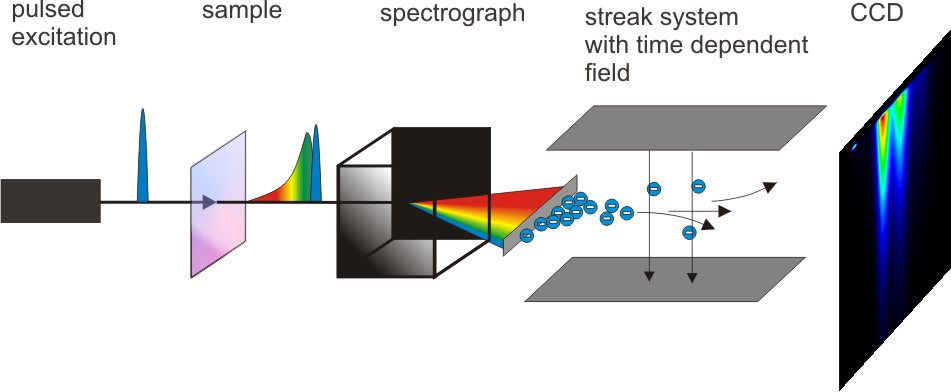
\includegraphics[width=0.75\textwidth]{./Chapter4/streakcam.jpeg}
\caption[Diagram of streak camera detection scheme.]{Following pulsed excitation of an emissive sample, PL photons are dispersed using a spectrograph and "streaked" across a CCD using a time dependent applied voltage sweep.}
\label{f:streakcam}
\end{center}
\end{figure}

Streak camera measurements are carried out utilizing a pulsed excitation source. First, a laser pulse excites a luminescent sample. Subsequent to photoexcitation, emitted PL photons are collected and spectrally resolved by a spectrograph. These photons are then directed through a streaking cathode onto a phosphor screen, producing flashes detected by a CCD. The streaking cathode utilizes a time-dependent voltage sweep synchronized with the laser excitation. As a result, electrons strike the target phosphor at a distinct and precise height which depends on the time after photoexcitation that they entered the streak cathode. The net result is a temporally and spectrally resolved image which may be binned vertically and horizontally to yield PL decay dynamics or time-resolved emission spectra, respectively.


\section{Observation of Acoustic Phonon Transport Using Ultrafast Photoluminescence Spectroscopy}

Significant information exists for CdSe NCs regarding carrier dynamics and electronic structure, the relevant findings of which we summarize here. Following photoexcitation, excitonic intraband relaxation down to the “band-edge” states takes place on subpicosecond to single-picosecond time scales \cite{PhysRevLett.80.4028, PhysRevB.60.R2181, PhysRevLett.96.057408}.  Radiative recombination, on the other hand, requires tens to hundreds of nanoseconds and exhibits strong temperature dependence owing to both details of the size- and shape-specific exciton fine structure as well as exciton-phonon interactions \cite{:/content/aip/journal/jcp/96/2/10.1063/1.462114, PhysRevLett.75.3728, PhysRevB.54.4843, PhysRevB.60.1819, :/content/aip/journal/apl/82/17/10.1063/1.1570923, doi:10.1021/jp051738b, PhysRevB.74.085320,PhysRevLett.102.177402}.  Crystal field effects, spin-orbit coupling, and the electron-hole exchange interaction \cite{PhysRevB.54.4843, PhysRevB.60.1819} give rise to the energetic ordering and size-dependent energy spacings of the band-edge exciton states. A dipole forbidden (optically passive or “dark”) lowest-energy exciton, with spin projection $J = \pm 2$ along the wurtzite c axis, resides below an optically allowed (bright, $J = \pm 1$) exciton state by 2 - 17 meV, with larger dark-bright splittings ($\Delta_{db}$) for smaller NC sizes \cite{PhysRevLett.75.3728}.  At cryogenic temperatures, insufficient thermal energy exists to populate the lowest-energy bright exciton state, and microsecond lifetimes result due to the weakly emissive character of the dark exciton. By contrast, at higher temperatures, a thermal (Boltzmann) population of bright excitons radiates with an established lifetime of $\sim 20$ ns \cite{:/content/aip/journal/apl/82/17/10.1063/1.1570923}.  Nirmal \emph{et al.} established values of $\Delta_{db}$ from the energy difference between a spectrally narrow excitation laser and the proximal, zero-phonon PL (PL) peak position owing to spin-forbidden recombination from dark excitons \cite{PhysRevLett.75.3728}.  The same study found LO-phonon-assisted emission bands at lower energy wherein emission of a photon and generation of an LO phonon yields momentum-conserving transitions from the dark state. Magnetic fields were found to quantum mechanically mix proximal bright and dark states, which increases the zero-phonon amplitude relative to the LO-phonon-assisted feature and yields a notable increase in the radiative recombination rate \cite{PhysRevLett.75.3728}.  Also, cryogenic four-wave mixing measurements suggest that optically bright photoexcited excitons decay into lowest-energy dark exciton states roughly in the same time as intraband relaxation \cite{PhysRevB.73.125322}.  \par

In this section, we examine a long-standing, poorly understood feature in CdSe NC dynamics and attribute it to thermal dissipation. Specifically, in addition to the more fully characterized dark and bright radiative lifetimes, Crooker showed that low-temperature time-resolved PL (trPL) measurements exhibit an unusual, rapid initial decay for sample temperatures below $\sim 20$ K, signatures of which appear in numerous reports \cite{:/content/aip/journal/jcp/96/2/10.1063/1.462114, :/content/aip/journal/apl/82/17/10.1063/1.1570923, doi:10.1021/jp051738b, PhysRevB.74.085320, PhysRevLett.102.177402}.  To date, this fast burst of PL has remained uncharacterized due to an instrumental lack of sufficient temporal resolution. We temporally and spectrally resolve this feature, revealing clear size-dependent dynamics as well as distinct spectral characteristics that, taken together in the context of literature from metals and semiconductors, permit us to assign the feature to size-dependent thermal outflow. While low temperatures are required in order to observe this outflow, the thermal transport constants may be scaled to temperatures of relevance to device applications.  \par

We examine several sizes of CdSe NCs capped with octadecylamine, which exhibit PL quantum yields in excess of 20\% at room temperature. Small discrepancies exist regarding available CdSe sizing curves (used to convert absorption maximum to NC radius), but these did not qualitatively impact presented results. NCs were dispersed in a 1:1 octadecane:eicosane solvent and dripped onto a sapphire substrate. The samples were loaded into a closed-cycle helium cryostat and photoexcited with 35 fs pulses from a 2 kHz amplified Ti-sapphire laser at 3 eV. The excitation fluence utilized corresponds to the production of less than 0.05 electron-hole pairs per NC per pulse, and results were unchanged for 3$\times$ higher or lower excitation intensities. PL photons were directed to a 150 mm spectrograph and streak camera. Detector regions were binned vertically or horizontally to produce time-resolved spectra or spectrally resolved dynamics, respectively. \par

A streak camera image recorded at 2.6 K [Fig. \ref{f:trpl1}(a)]  for the first few hundred picoseconds following photoexcitation of a 1.6-nm-radius NC sample (556 nm 1S absorbance maximum) shows a fast initial burst of emission that is not distinct at 80 K [Fig. \ref{f:trpl1}(b)], in qualitative agreement with previous reports that did not spectrally or temporally resolve this feature \cite{:/content/aip/journal/apl/82/17/10.1063/1.1570923, doi:10.1021/jp051738b, PhysRevB.74.085320, PhysRevLett.102.177402}.  At 2.6 K, time-resolved spectra [Fig. \ref{f:trpl1}(c)] exhibit shorter wavelength PL during the first $\sim$ 80 ps following excitation which redshifts to a constant value for longer times, whereas the 80 K sample temperature lacks any pronounced spectral shift over the same time range. Dynamics in Figs. \ref{f:trpl1}(e) and \ref{f:trpl1}(f) display a fast relaxation feature at 2.6 K for bluer wavelengths that is largely absent from the redder PL at 2.6 K and is absent for all wavelengths in the 80 K data. \par

\begin{figure}
\begin{center}
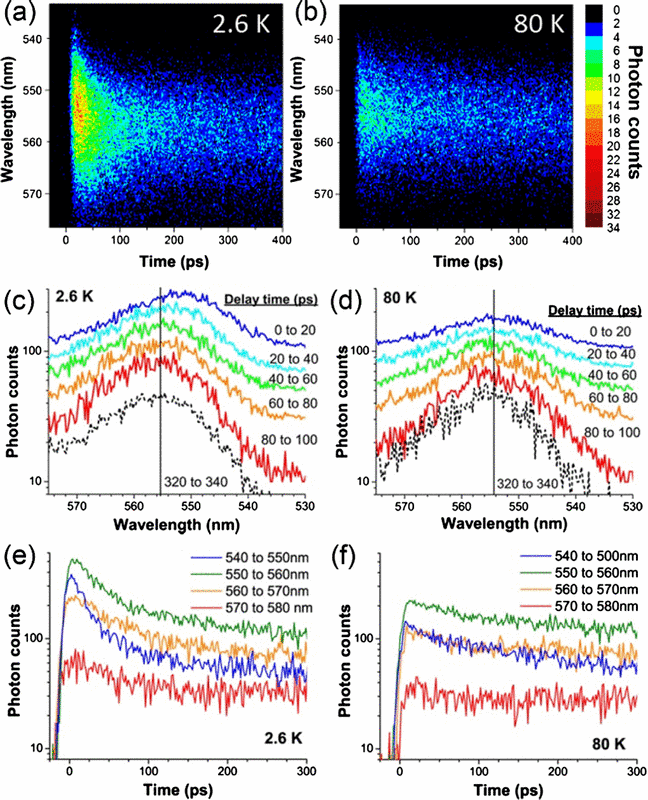
\includegraphics[width=0.75\textwidth]{./Chapter4/trpl1.png}
\caption[Spectra and dynamics of PL at 3K and 80K from an ensemble of CdSe NCs.]{(a) Temporally and spectrally resolved single exciton PL from a 1.6-nm-radius CdSe NC ensemble at 2.6 K and (b) at 80 K. Here, lower sample temperature results in a faster emission feature as well as a spectral shift to lower energy with time. (c),(d) Time-resolved spectra collected at the indicated temperatures and binned over the indicated time delays reveal a redshift with increasing time at 2.6 K that is not observed at 80 K. Spectra are linearly offset for clarity. The black vertical lines indicate the peak emission amplitude of the 320-340 ps time-binned spectrum. (e),(f) Spectrally resolved PL dynamics become biexponential for shorter PL wavelengths in the case of the lower sample temperature.}
\label{f:trpl1}
\end{center}
\end{figure}

Single Gaussian fits of the ensemble-broadened spectra shown in Fig. \ref{f:trpl1}(c) yield similar full width at half maximum linewidths (16.2 nm for $t = 0 - 20$ ps and 17.3 for $t = 320 - 340$ p), which suggests that a single population evolves to emit with reduced energy over time. For the dynamics collected at 2.6 K in Fig. \ref{f:trpl1}(e), we find that the decay on the blue side of the PL is well-described by a biexponential decay, while the redder PL dynamics at low temperature and all of the dynamics recorded at 80 K appear single exponential in the time window examined. The biexponential fit time constants differ by more than 1 order of magnitude, which allows for highly independent fits. While the spectrally resolved dynamics in Fig. \ref{f:trpl1}(e) each exhibit fast decay constants that differ by $\sim$25\% for proximal spectral slices (slower for lower-energy PL), most of the fast-component amplitude is present in a narrow spectral region. To systematically compare data for different samples, we hereafter bin all trPL to the blue of the time-integrated PL spectral maximum so as to yield characteristic (“blue-side”) dynamics of the higher energy, prompt emission. \par

In Fig. \ref{f:trpl2}, we display temporally resolved blue-side decay dynamics, normalized at late times, for multiple NC sizes at both 2.6 and 80 K. For each sample, the low-temperature dynamics become faster and biexponential in comparison to the slower single exponential decays recorded at high temperature. We summarize two general trends in \ref{f:trpl3}: The blue side becomes progressively longer-lived as the NC radius increases, and the spectral shift associated with the fast decay feature yields a roughly constant value of $\sim$25 meV irrespective of NC size (inset).  The fast decay lifetime plotted vs NC radius squared exhibits a linear relationship. While such a trend has not been reported previously for a semiconductor NC composition, a comparable relation has been found in metal nanoparticles \cite{doi:10.1021/jp020581+, PhysRevB.66.224301} and is attributed to particle thermalization rates as dictated by interfacial and thermal diffusion \cite{doi:10.1021/jp020581+, PhysRevB.66.224301,doi:10.1021/jp048375k}. \par

\begin{figure}
\begin{center}
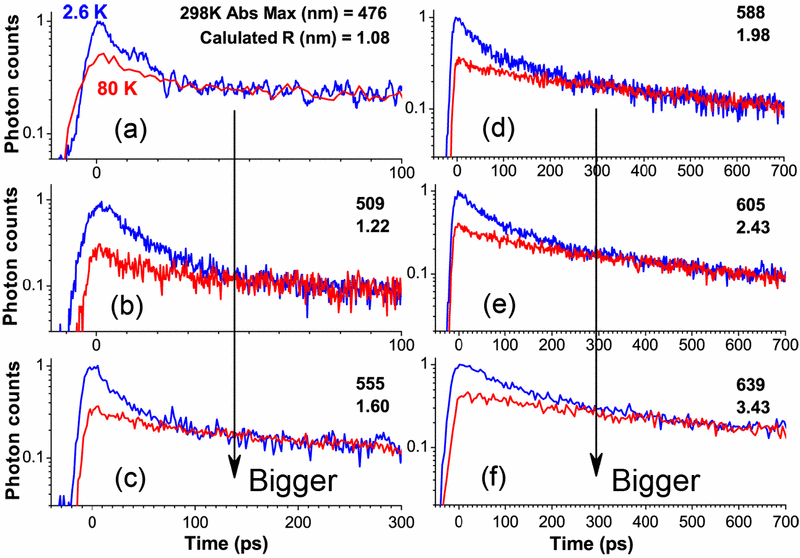
\includegraphics[width=0.75\textwidth]{./Chapter4/trpl2.png}
\caption[High-energy PL decay dynamics for various sizes of CdSe NC at 3K and 80K.]{“Blue-side” radiative recombination dynamics for CdSe samples with indicated radii generated for the higher energy half of the time-integrated PL spectrum at 2.6 (blue lines) and 80 K (red lines). Traces were scaled to overlap at long time. For every sample, the low-temperature trPL data become biexponential. Also, the decay feature appearing at low temperature becomes increasingly faster with reduced NC radius. Note that the tick mark step size is constant (100 ps) for each data panel and that the measured time window is larger for larger NC size.}
\label{f:trpl2}
\end{center}
\end{figure}

\begin{figure}
\begin{center}
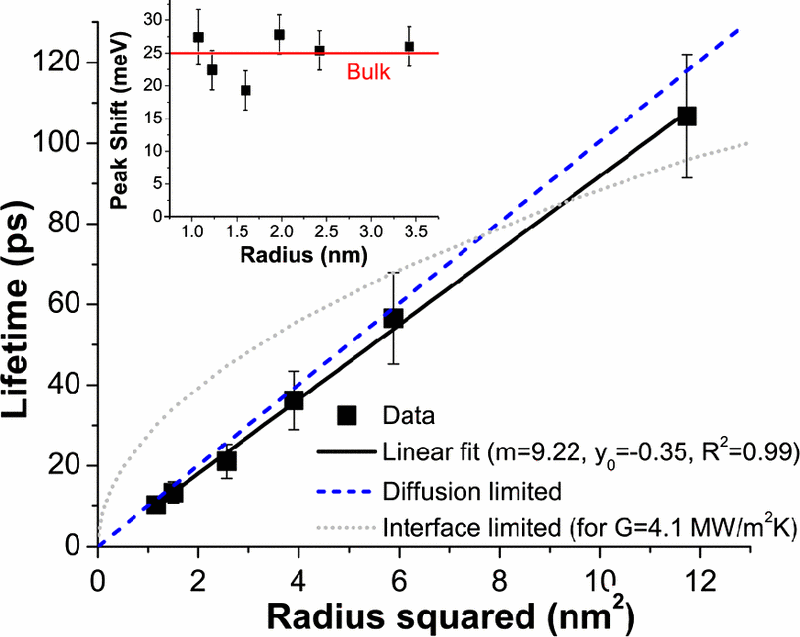
\includegraphics[width=0.75\textwidth]{./Chapter4/trpl3.png}
\caption[Fast pholuminescence feature lifetimes as a function of CdSe nanocrystal radius.]{The faster decay time derived from biexponential fits of the trPL data in Fig. \ref{f:trpl2} (squares) exhibits a linear relationship with the NC radius squared (fitted black solid line). Calculations of diffusion-limited (blue dashed line) and interfacial-conductance-limited (gray dotted line, estimated for an interfacial conductance of 4.1 $MW/m^2K$) dissipation suggest that diffusion controls the measured decay times. The inset displays the energy difference between early recombination and emission subsequent to the fast initial decay. The spectral shifts for multiple NC radii are fairly constant and comparable to the 25-meV LO-phonon energy of bulk CdSe (solid red line). Recombination from higher lying states in the CdSe NC exciton fine structure is not apparent, since such emission would exhibit strong size dependence corresponding to $\Delta_{db}$ values ranging from 2 to 17 meV for the NC size range probed.}
\label{f:trpl3}
\end{center}
\end{figure}

Next, we probe the temperature dependence of the trPL collected for the 1.6-nm-radius sample.  Figure \ref{f:trpl4}(a) shows that the amplitude of the fast decay feature remains unchanged between 2.6 and 10 K but that higher temperatures cause the fast-feature amplitude to decrease. To highlight the evolution of the fast vs slow decay, Fig. \ref{f:trpl4}(b) displays the temperature-dependent ratio of instantaneous PL intensity binned from $t = 0 - 5$ ps divided by that from $t = 200 - 205$ ps for three CdSe NC sizes. Such ratios evolve with temperature similar to Boltzmann thermal partitioning with characteristic energies of 2.2, 1.5, and 1.0 ($\pm$ 0.1) meV for 1.2-, 1.6-, and 2.4-nm radii, respectively, in agreement with calculated lowest-energy acoustic phonon modes in CdSe NCs \cite{PhysRevLett.102.177402, doi:10.1021/nl061414e}. \par

\begin{figure}
\begin{center}
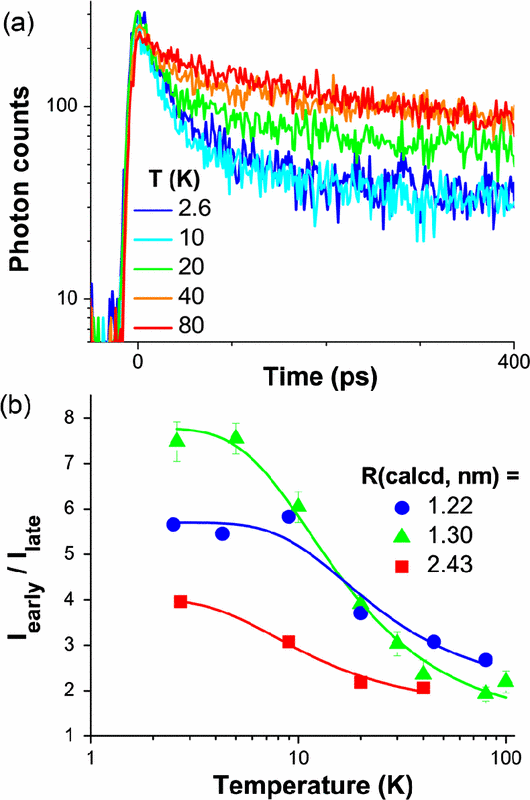
\includegraphics[width=0.65\textwidth]{./Chapter4/trpl4.png}
\caption[Temperature dependent decay of high energy PL from CdSe nanocrystals.]{(a) Increasing sample temperature results in a decrease in amplitude of the fast dynamical component, here for a 1.6-nm-radius CdSe NC sample. (b) The ratio of instantaneous PL intensities integrated from $t = 0 - 5$ ps ($I_{early}$) and from $t = 200 - 205$ ps ($I_{late}$) taken from dynamics such as those shown in (a) for three CdSe NC sizes suggests that Boltzmann populations of low-energy phonons in the NCs eliminates the fast relaxation feature for sufficiently high temperatures. Lines show appropriately scaled thermal partitioning of NCs lacking acoustic phonon excitation, as described in the text. Representative error bars are shown for the 1.30-nm-radius NC sample.}
\label{f:trpl4}
\end{center}
\end{figure}

In the respective contexts of wave packet decoherence and intraband relaxation, Scholes \cite{doi:10.1021/nl061414e, doi:10.1021/nl803275a, :/content/aip/journal/jcp/132/10/10.1063/1.3350871} and Prezhdo and co-workers \cite{doi:10.1021/jp0669052} recently proposed that acoustic phonons transiently mix dark and bright exciton states. In the picture presented by these authors, nonequilibrium acoustic phonons, generated in the current studies as a result of exciton intraband relaxation, mechanically distort the NCs and perturb the fine structure, which increases the oscillator strength of the lowest-energy dark exciton state. At the low temperatures examined in this work, the observed radiative recombination rate diminishes with time as these phonons leave the NCs. By contrast, for higher temperatures, there is a significant equilibrium population of acoustic phonons in the NCs. Furthermore, the increase of the fast-feature amplitude with decreasing temperature, explored in Fig. \ref{f:trpl4} follows the equilibrium thermal partition function describing NCs that lack acoustic phonon population. This relationship suggests that a single, lowest-energy equilibrium acoustic phonon is sufficient to preclude observation of the fast relaxation feature. Subsequent to acoustic phonon dissipation for low temperatures, the radiative rate decreases and LO-phonon-assisted recombination dominates the ensemble PL spectrum, resulting in the size-independent redshift. Acoustic phonon-induced mixing is also consistent with both a notable lack of magnetic circular dichroism at early times following excitation, as reported by Furis et al. \cite{doi:10.1021/jp051738b},  as well as the temperature-dependent radiative recombination rates reported by Oron et al. \cite{PhysRevLett.102.177402} \par

Next we focus on thermal transport estimates, first for a relatively large, 3-nm-radius particle (for which bulk constants may be fairly accurate) and then as a function of NC size. Thermal transport models consider two regimes of heat dissipation: thermal diffusion controlled or interfacial conductivity controlled, each of which can dictate the time scale as well as the functional dependence on NC radius $R$.  We utilize the work of Ge, Cahill, and Braun \cite{PhysRevB.66.224301} to estimate dissipation time scales specific to a CdSe NC suspended in an octadecane matrix initially at 10 K excited with 1 eV of photon energy in excess of the band gap. Modeling the CdSe NC as a Debye solid ($C$ follows $T^3$) reveals that the provided photon excess energy increases the temperature to $\sim$16 K for a 3-nm-radius particle (presented results were insensitive to the initial NC temperature at least within the range of 2.6-10 K).  \par

For large thermal conductivity at the CdSe-alkane interface, thermal diffusion in the medium surrounding the NCs would dictate thermalization time and should follow $\tau_d = \left(C_p\rho_pR\right)^2/9C_m\rho_m\Lambda_m$, where, for the particle ($p$) and matrix ($m$), $C$ is specific heat, $\rho$ is density, and $\Lambda$ is linear thermal conductivity [utilized constants include $C_{p, initial}\left(10 K\right) = 0.012$ J/gK, $C_p\left(16 K\right) = 0.061$ J/gK, $C_m\left(10 K\right) = 0.011$ J/gK, $\rho_p = 5.65$ g/cm$^3$, $rho_m = 0.777$ g/cm$^3$, and $\Lambda_m = 0.0015$ J/cm Ks].  For a 3-nm-radius NC, we estimate a diffusion cooling time under our experimental conditions of 90 ps (close to the interpolated 83 ps).  Figure \ref{f:trpl3} shows close agreement between diffusion-limited cooling times and experiment. \par

In the scenario of rapid diffusion, conductance of heat through the CdSe-alkane interface limits thermalization time, and heat transport would obey $\tau_i = C_p\rho_pR/3G$, where $G$ is an unknown interfacial thermal conductivity.  Equating $\tau_i$ with the fitted data for a 3-nm-radius NC then yields $4.1$ MW/m$^2$K for $G$, which is 2 orders of magnitude smaller than the values obtained for metal nanoparticle dispersions \cite{doi:10.1021/jp020581+, PhysRevB.66.224301, doi:10.1021/jp048375k}.  However, as can be seen in Fig. \ref{f:trpl3} the functional dependence of $\tau_i$ appears inconsistent with the measured lifetimes, suggesting that interface conductance does not limit thermal transport for the samples studied and that the true value of $G$ is significantly higher than this estimate. \par

In conclusion, we reveal a new size-dependent trend in the dynamics of CdSe NCs despite more than two decades of study in this material. We show that low-temperature trPL exhibits faster subnanosecond decay for smaller NC size, attribute this trend to acoustic phonon dissipation, and denote consistency of the size-dependent decay times with a diffusion-limited thermal transport process. The rapid emission is accompanied by bluer PL photons, which we attribute to acoustic phonon-assisted relaxation. We ascribe a size-independent redshift with time to reliance of dark exciton radiative recombination on LO-phonon assistance subsequent to acoustic phonon dissipation. Our findings impact the picture of truly Boltzmann-populated bright and dark excitons at elevated temperatures, suggesting that acoustic phonon derivative coupling provides optoelectronically relevant mixing of exciton fine structure character. Perhaps more importantly, we present a means to characterize heat flow rates involving semiconductor nanoparticles and provide evidence that thermal dissipation from the nanoparticles is determined by thermal diffusion in the surrounding material rather than thermal impedance at the nanocrystal interface. These studies may offer means to intelligently design both low thermal conductivity nanomaterials for efficient thermoelectric power generation and high conductivity materials for stable device operation at elevated temperatures.

\section{Modeling Thermal Transport Using Non-Equilibrium Molecular Dynamics Simulations}

\subsection{Overview}

Numerous studies have applied MD simulations to the calculation of interfacial thermal conductance in nanoscale systems containing a solid, a chemical passivating layer, and/or a matrix material. However, much of this work focuses on systems where the solid is metallic, such as self-assembled alkanethiol monolayers on gold surfaces \cite{doi:10.1021/jp2073478, luo2010equilibrium, Luo20101}, gold nanoparticles \cite{doi:10.1021/jp410054j, doi:10.1021/ct500221u}, or nanocrystal arrays containing ligand-passivated gold building blocks \cite{ong2013surface, doi:10.1021/jp4120157}.  To date, no theoretical study and few experimental studies have examined the interfacial thermal conductance of semiconductor-organic systems common to the colloidal preparations described above, such as metal chalcogenides. Here, we apply reverse nonequilibrium MD (RNEMD) simulations to the calculation of interfacial thermal conductance in hexane-solvated, hexylamine-passivated CdSe interfaces, an extremely common experimental configuration for colloidal SNCs. First, we demonstrate that a simple potential originally parametrized by Rabani \cite{:/content/aip/journal/jcp/116/1/10.1063/1.1424321} to reproduce structural transformations and phonon dispersion relations is also capable of accurately describing thermal conductivity in CdSe. With a suitable potential for the modeling of thermal processes, we then examine interfacial thermal conductance for interfaces presenting the four wurtzite surfaces common to CdSe nanostructures: the $11\bar{2}0$ and $10\bar{1}0$ surfaces, which are nonpolar, and the $0001$ and $000\bar{1}$ surfaces, which are polar.  The role played by surface passivation is examined and estimates of interfacial thermal conductance are obtained for realistic CdSe interfaces. Furthermore, we examine the important role played by surface atomic density in establishing upper limits on the interfacial thermal conductance.

\subsection{Methodology}

A variety of theories exist for the calculation of interfacial thermal conductance (henceforth denoted $G$) from MD simulations. Time-correlation functions, such as the heat flux autocorrelation function (HFACF), can be computed from the results of equilibrium MD (EMD) simulations. These time-correlation functions can be used to compute various transport coefficients for the system being simulated, including the interfacial thermal conductance. However, EMD-based methods typically exhibit slow convergence of the HFACF for systems containing grain boundaries and low interfacial thermal conductance \cite{PhysRevB.65.144306}, as might be expected of a system containing acoustically mismatched components. Nonequilibrium MD (NEMD) methods can be preferable in such cases as less simulation time is required to achieve the steady-state temperature gradient necessary to compute $G$. Traditionally, NEMD methods impose a gradient on a simulation cell and measure the resulting flux, which can then be used to compute transport properties. However, as it is not apparent what type of gradient should be enforced at interfaces, RNEMD methods are better suited to the study of such systems. In RNEMD simulations of thermal conductivity, an unphysical heat flux is imposed between different regions of the simulation cell. The system responds by developing a temperature gradient between those regions. The resulting temperature gradient can be then be used to compute thermal conductivity as well as G. RNEMD approaches have been applied successfully to metal/organic systems in the past \cite{doi:10.1021/jp2073478,luo2010equilibrium,Luo20101,doi:10.1021/ct500221u} and will be used here for the study of semiconductor (CdSe)/organic systems. The RNEMD simulations in this work utilize a velocity shearing and scaling (VSS) algorithm, the details of which are reported below. \par

\subsubsection{VSS-RNEMD}

The original momentum swapping procedure developed by M{\"u}ller-Plathe \cite{:/content/aip/journal/jcp/106/14/10.1063/1.473271, PhysRevE.59.4894} generally works well for describing the thermal conductivity of bulk liquids, but exchange moves perturb the system away from thermal distributions and at large momentum flux values, the resulting “notched” temperature gradients fall outside of the linear response regime required in order to utilize Fourier’s law in the derivation of $G$ \cite{:/content/aip/journal/jcp/132/1/10.1063/1.3276454}.  To address these issues, we utilize a recently developed VSS technique which applies velocity shearing and scaling exchanges between the two slabs \cite{doi:10.1080/00268976.2012.680512}.  Such exchanges are subject to a set of constraints which ensure that new configurations are sampled from an NVE (constant N, V, and energy, E) ensemble. In comparison to the original M{\"u}ller-Plathe method, VSS-RNEMD distributes flux more evenly within the exchange regions and avoids strong perturbations. The enforcement of thermal sampling and wide distribution of imposed flux reduces the development of nonlinear temperature gradients. Furthermore, the VSS-RNEMD method can create a flux between atoms of arbitrary identity without efficiency losses due to differences in particle mass, making VSS-RNEMD an ideal method for heterogeneous systems \cite{doi:10.1080/00268976.2012.680512}.  \par

In VSS-RNEMD simulations, a flux is imposed by periodically shifting and scaling particle velocities ($\vec{v}_i$ and $\vec{v}_j$) in two regions (denoted H for hot and C for cold) separated by half the length of the simulation cell in the intended flux axis.  Equations \ref{eq:rnemd_eqS1} and \ref{eq:rnemd_eqS2} describe this operation mathematically.
\begin{equation} \label{eq:rnemd_eqS1}
\vec{v}_i \leftarrow  c \cdot \left(\vec{v}_i - \left\langle\vec{v}_c\right\rangle\right) + \left(\left\langle\vec{v}_c\right\rangle + \vec{a}_c\right)
\end{equation}
\begin{equation} \label{eq:rnemd_eqS2}
\vec{v}_j \leftarrow  h \cdot \left(\vec{v}_i - \left\langle\vec{v}_h\right\rangle\right) + \left(\left\langle\vec{v}_h\right\rangle + \vec{a}_h\right)
\end{equation}
In Eq. \ref{eq:rnemd_eqS1} and \ref{eq:rnemd_eqS2}, $\left\langle\vec{v}_c\right\rangle$ and $\left\langle\vec{v}_h\right\rangle$ are the average velocities in the C and H slabs, respectively.  Each particle receives an incremental change to its velocity via the $\vec{a}$ terms, which are governed by the imposed momentum flux $j_z(\vec{p})$:
\begin{equation} \label{eq:rnemd_eqS3}
\vec{a}_c = -\frac{j_z\left(\vec{p}\right)\Delta t}{M_c}
\end{equation}
\begin{equation} \label{eq:rnemd_eqS4}
\vec{a}_c = +\frac{j_z\left(\vec{p}\right)\Delta t}{M_h}
\end{equation}
In Eq. \ref{eq:rnemd_eqS3} and \ref{eq:rnemd_eqS4}, $M_{h\left(c\right)}$ is the total mass of particles in the hot (cold) slab, and $\Delta t$ is the time interval between two VSS operations.  The scaling constants $c$ and $h$ are given by solutions to energy conservation constraints which are described by Equations \ref{eq:rnemd_eqS5} and \ref{eq:rnemd_eqS6}: 
\begin{equation} \label{eq:rnemd_eqS5}
K_c - J_z\Delta t = c^2\left(K_c -\frac{1}{2}M_c\left\langle\vec{v}_c\right\rangle^2\right) + \frac{1}{2}M_c\left(\left\langle\vec{v}_c\right\rangle + \vec{a}_c\right)^2
\end{equation}
\begin{equation} \label{eq:rnemd_eqS6}
K_h + J_z\Delta t = c^2\left(K_h -\frac{1}{2}M_h\left\langle\vec{v}_h\right\rangle^2\right) + \frac{1}{2}M_h\left(\left\langle\vec{v}_h\right\rangle + \vec{a}_h\right)^2
\end{equation}
In Eq. \ref{eq:rnemd_eqS5} and \ref{eq:rnemd_eqS6}, $K_{h\left(c\right)}$ is the translational kinetic energy of the hot (cold) slab.  Simultaneous solution of Eq. \ref{eq:rnemd_eqS5} and \ref{eq:rnemd_eqS6} yields the scaling coefficients $c$ and $h$ and ensures that the simulation samples from from an NVE ensemble.  At each time interval, $c$, $h$, $\vec{a}_c$, and $\vec{a}_h$ are solved for subject to the imposed momentum flux $j_z\left(\vec{p}\right)$ and the imposed thermal flux, $J_z$.  Following solution for these variables, velocity scaling steps are applied accoridng to Eq. \ref{eq:rnemd_eqS1} and \ref{eq:rnemd_eqS2}.  Eventually, the simulation develops a thermal gradient in response to the applied flux, which is in turn utilized derive the thermal transport properties of the system, as detailed below. 

\subsubsection{Analysis of VSS-RNEMD Simulations}

As described above, an unphysical heat flux $J_z$ is imposed between "hot" and "cold" regions in the simulation cell, with the exchange axis denoted $Z$.  Eventually, a steady-state temperature gradient develops between the two regions. Using the slope of this temperature gradient, it is simple to obtain the thermal conductivity of the simulation cell, denoted $\lambda$, using Equation \ref{eq:rnemd1}:
\begin{equation} \label{eq:rnemd1}
J_z = -\lambda\left(\frac{\partial T}{\partial Z}\right)
\end{equation}
For systems containing one or more interfaces, the regions on either side of an interface will develop relatively homogeneous, but distinct, temperatures. The temperature difference at these interfaces can be used to derive the interfacial thermal conductance, $G$, as shown Equation \ref{eq:rnemd2}:
\begin{equation} \label{eq:rnemd2}
G = \frac{J_z}{\Delta T}
\end{equation}
While other definitions, formulated in terms of temperature derivatives, exist for the interfacial thermal conductance, the form shown in Eq. \ref{eq:rnemd2} was shown to be both straightforward in its application and in good agreement with experimental values for a gold-alkanethiol interface \cite{doi:10.1021/jp2073478}.  It is this form which we will utilize in the work detailed below. In systems containing multiple interfaces, this method can be applied by calculating the total thermal boundary resistance ($R_K$, the inverse of $G$) for a series of thermal resistors:
\begin{equation} \label{eq:rnemd3}
G^{-1} = R_K = \sum_{i = 1}^n R_i = \sum_{i = 1}^n \frac{T_{i+1} - T_i}{J_z} = \frac{T_n - T_1}{J_z}
\end{equation}

\subsubsection{Interaction Potentials}
It is necessary to demonstrate the suitability of any interaction potential used in a classical MD simulation for simulating the physical properties or processes of interest. In his original work, Rabani fitted Coulombic and Lennard-Jones potential energy parameters to reproduce the elastic constants and phonon dispersion relations of CdSe \cite{:/content/aip/journal/jcp/116/1/10.1063/1.1424321}.  The form of the interaction potential is shown in Equation \ref{eq:rnemd4}:
\begin{equation} \label{eq:rnemd4}
V_{ij} = \left(\frac{q_iq_j}{r_{ij}}\right) + 4\epsilon_{ij}\left[\left(\frac{\sigma_{ij}}{r_{ij}}\right)^{12}- \left(\frac{\sigma_{ij}}{r_{ij}}\right)^6\right]
\end{equation}
In Eq. \ref{eq:rnemd4}, $q_i$ is the charge on atom $i$, $r_{ij}$ is the distance between atoms $i$ and $j$, $\epsilon_{ij}$ is the depth of the potential energy well, and $\sigma_{ij}$ is the distance at which the interparticle potential is zero.  The Rabani interaction potential has been shown to reproduce well the Hamaker constant of bulk CdSe as well as the pressure-induced phase transition from the ambient-pressure wurtzite to the high-pressure rocksalt phase \cite{:/content/aip/journal/jcp/116/1/10.1063/1.1424321}.  The Rabani potential has also been shown to accurately capture the transition of CdSe nanostructures from a wurtzite to rocksalt phase at pressures elevated relative to the bulk transition \cite{PhysRevLett.96.255701, doi:10.1021/nl3007165}.  Furthermore, the Rabani potential has been shown to accurately reproduce the size-dependent phonon frequencies and electron-phonon coupling (based on an effective-mass wave function model) in CdSe nanoparticles \cite{doi:10.1021/nn201475d}.  Here, we demonstrate the applicability of the Rabani potential to the calculation of thermal conductivity in bulk CdSe.  Figure \ref{f:rnemd1}(a) shows the temperature gradient developed during a RNEMD simulation of a 30 Å × 30 Å × 400 Å slab of wurtzite CdSe. A target flux of 695 MW/m$^2$ was imposed, with kinetic energy exchanges occurring every 5 fs.  \ref{f:rnemd1}(b) displays the inverse of thermal conductivity values displayed for a range of system lengths having an identical cross-section. As the finite size of the simulation cell artificially truncates the phonon mean free path compared to a true bulk system, it is necessary to account for finite size effects \cite{chantrenne2004finite}.  A linear fit of this data, shown as a dotted line in \ref{f:rnemd1}(b), may be used to extrapolate to the true bulk thermal conductivity, as shown by Equation \ref{eq:rnemd5}:
\begin{equation} \label{eq:rnemd5}
\frac{1}{\lambda\left(\infty\right)} = \frac{1}{\lambda\left(L\right)} + \frac{C}{L}
\end{equation}
In Eq. \ref{eq:rnemd5}, $\lambda$ is the thermal conductivity, $C$ is a constant, and $L$ is the length of the simulation cell along the kinetic energy flux direction. Extrapolation to infinite length yields a thermal conductivity of 6 $\pm$ 2 W/m/K, which is firmly within the range of experimental thermal conductivity values (4 - 9 W/m/K) reported for bulk, crystalline CdSe at 300 K \cite{berger1996semiconductor, PhysRevB.6.3791, doi:10.1021/nl400531f}.  \par

\begin{figure}
\begin{center}
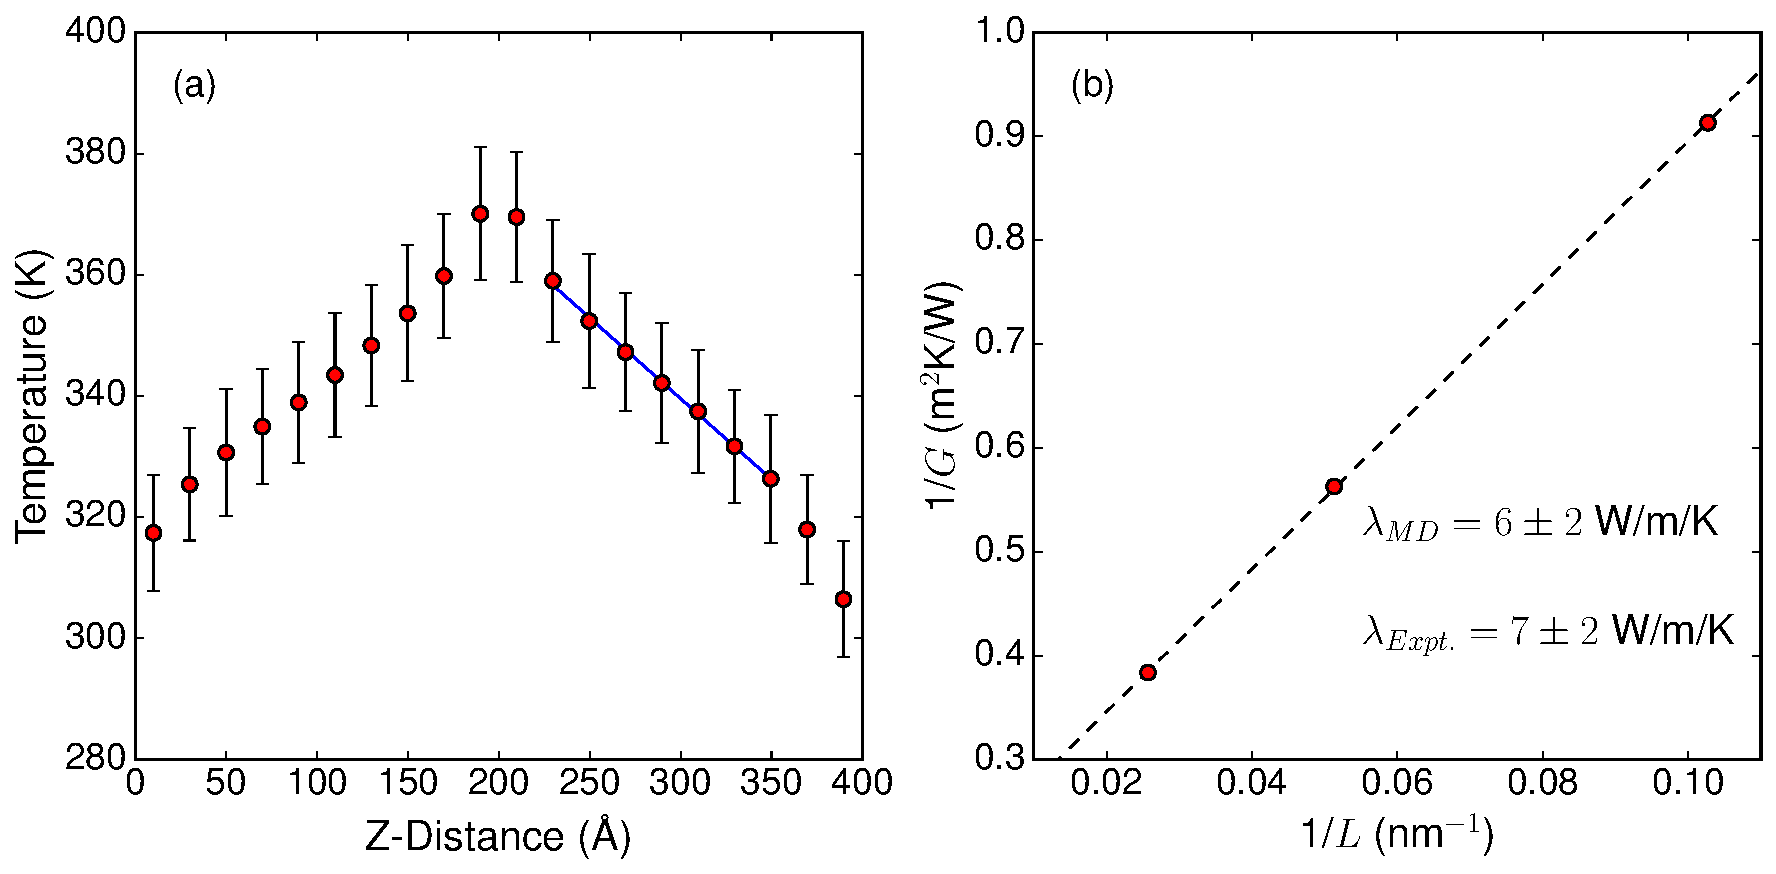
\includegraphics[width=\textwidth]{./Chapter4/rnemd1.pdf}
\caption[Determination of thermal conductivity in bulk CdSe via MD simulation.]{(a) Temperature profile along the kinetic energy exchange axis obtained following a 3 ns RNEMD simulation of a wurtzite CdSe slab. Error bars are derived from temperature deviations in each bin along the production trajectory. The solid blue line indicates a linear fit to the linear response region of the temperature profile. The slope of this line is used to obtain thermal conductivity via Eq. \ref{eq:rnemd1}.  (b) Inverse thermal conductivity (obtained as described above) as a function of inverse length. Extrapolation to the y-intercept yields the bulk (i.e., infinite length) thermal conductivity. Simulated ($\lambda_{MD}$) and experimental ($\lambda_{expt}$) values of thermal conductivity are given on the figure. Uncertainty values for $\lambda_{MD}$ were obtained from the average of four statistically independent RNEMD simulations, while the standard deviation in $\lambda_{expt}$ is obtained from an average of reported literature values \cite{berger1996semiconductor, PhysRevB.6.3791, doi:10.1021/nl400531f}.}
\label{f:rnemd1}
\end{center}
\end{figure}

To address the organic components of the system, our simulations utilize a combination of united-atom (UA) and explicit hydrogen (EH) parameters for the TraPPE force field \cite{doi:10.1021/jp0504827}.  The TraPPE model includes parametrizations for bonding interactions including stretches, bends, dihedrals, and torsions. For the amine terminal of the hexylamine molecules, TraPPE-EH parameters were used to model N and explicit H atoms to account for any role played by H in determining the packing of ligand monolayers on the CdSe surface. All other hydrocarbons utilized the TraPPE-UA model. Previous simulations of thermal conductivity which compared a similarly parametrized all-atom force field (the Optimized Potentials for Liquid Simulations - All Atom, or OPLS-AA \cite{jorgensen1988opls}) to the TraPPE-UA did not find a significant difference in the thermal conductivity obtained from RNEMD simulations between the two force fields. Thus, the TraPPE-UA models are computationally efficient while maintaining accuracy \cite{doi:10.1021/jp2073478}.  \par

\subsubsection{Simulation Protocol}

To construct CdSe surface/solvent interface models, a slab of crystalline (wurtzite) CdSe having a fixed cross-section of 30 \r{A}  $\times$ 30 \r{A} was built having a particular crystalline direction oriented along the z-axis of the simulation cell and then equilibrated at 200 K and 1 atm. For the systems studied here, 125 ps of equilibration time was found to be sufficient to ensure stable thermodynamic variables. Following equilibration in the NPT and NVT ensembles, the simulation cell was expanded along the z-axis to twice the length of the wurtzite slab. This empty space was filled with hexane molecules to experimental density at 200 K using the PackMOL algorithm \cite{JCC:JCC21224}.  The simulation cell was then equilibrated again at 200 K and 1 atm first in the NPT and then NVT ensemble. After all equilibration steps were complete, RNEMD simulations were run in the NVE ensemble using a target flux of 695 MW/m$^2$ and exchange time of 5 fs. RNEMD simulations were run for sufficiently long times to ensure the development of a stable temperature profile, typically 3 ns. \par

Passivated CdSe surfaces were constructed in a similar fashion. Hexylamine, a common experimental passivating ligand, was chosen for this study. Passivated CdSe surfaces were constructed by placing a hexylamine molecule, initially aligned along the z-axis of the simulation cell, atop each grafting site on the surface.  For the $11\bar{2}0$, $10\bar{1}0$, and $0001$ surfaces, hexylamine was initially placed top Cd atoms, while for the $000\bar{1}$ surface, which is Se terminated, hexylamine was placed atop Se atoms.  These placements are in agreement with DFT studies, which indicate that amine surface ligands primarily interact with surface Cd atoms \cite{doi:10.1021/jp064051f, doi:10.1021/jp903291d}.  After ligand placement, the system was equilibrated in an NVT ensemble to permit internal relaxation followed by equilibration at 200 K and 1 atm in the NPT ensemble. After these equilibration steps, the simulation cell was expanded to twice the length of the wurzite + ligand system and filled with hexane as before. The system was then equilibrated again at 200 K and 1 atm in the NPT and then NVT ensembles. Following these equilibration steps, RNEMD simulations were executed as described above. Ligand motion is unconstrained throughout the simulation; ligand molecules are free to sample the CdSe surface. Ligand migration occurs on the $000\bar{1}$ surface during equilibration, with ligand headgroups shifting to the interstitial sites in between surface Se atoms, situated roughly halfway between the surface Se atom and subsurface Cd atom below it. At the same time, these subsurface Cd atoms relax toward the surface. Ligand migration is minimal for the other surfaces studied here. All of the MD simulations in this work utilized the OpenMD software package \cite{gezelter2010openmd}.

\subsection{Results and Discussion}
Having established above that the Rabani interaction potential is well-suited for the simulation of thermal conductivity in bulk wurtzite CdSe, we now simulate the interfacial thermal conductance of various CdSe surfaces passivated and solvated by organic ligands.  Figure \ref{f:rnemd2}(a) details the chemically distinct components used to model solvent molecules in the simulations presented here.  The temperature profile resulting from a 3 ns RNEMD simulation of a CdSe($11\bar{2}0$)/hexane interface is shown in Figure \ref{f:rnemd2}(b).  Utilizing Eq. \ref{eq:rnemd2}, we obtain an interfacial thermal conductance of $\sim$8 MW/m$^2$/K for a 40 \r{A} long slab.  As with simulations of infinite, bulk materials, RNEMD simulations show convergence in the interfacial thermal conductance with respect to the size of the system. The dependence of $G$ on slab thickness arises from the disordering of atoms near the interface, resulting in an altered vibrational power spectrum with respect to the bulk atoms. In thin slabs, all atoms are close to an interface and therefore exhibit similar vibrational power spectra. This similarity yields higher $G$ values for thinner slabs. To isolate finite size effects from interfacial conductance, we performed RNEMD simulations on a series of slab lengths. The length of the hexane portion of the simulation cell was increased proportionally in each simulation. A fitting procedure similar to Eq. 5 \ref{eq:rnemd5} may be used to obtain $G$  values for a CdSe/hexane interface propagating to infinite length in the kinetic energy flux direction on either side of the interface.  Figure \ref{f:rnemd2}(c) displays the $G$ value obtained for 3 CdSe($11\bar{2}0$) slabs of increasing thickness.  The inset of Fig. \ref{f:rnemd2}(c) displays a snapshot of the CdSe($11\bar{2}0$)/hexane interface, taken from one of the trajectories used to produce the data.  Similar simulations were performed for the $10\bar{1}0$, $000\bar{1}$, and $0001$ surfaces.  These surfaces are of particular interest as they are the exposed surfaces of most CdSe nanocrystals \cite{doi:10.1021/nl0485861}.  Each of the surfaces yields a similar value for the interfacial thermal conductance (2 - 3.5 MW/m$^2$/K).  The results of our calculations for a bare CdSe/hexane interface are summarized in Table \ref{table:rnemdT1}. \par

\begin{figure}
\begin{center}
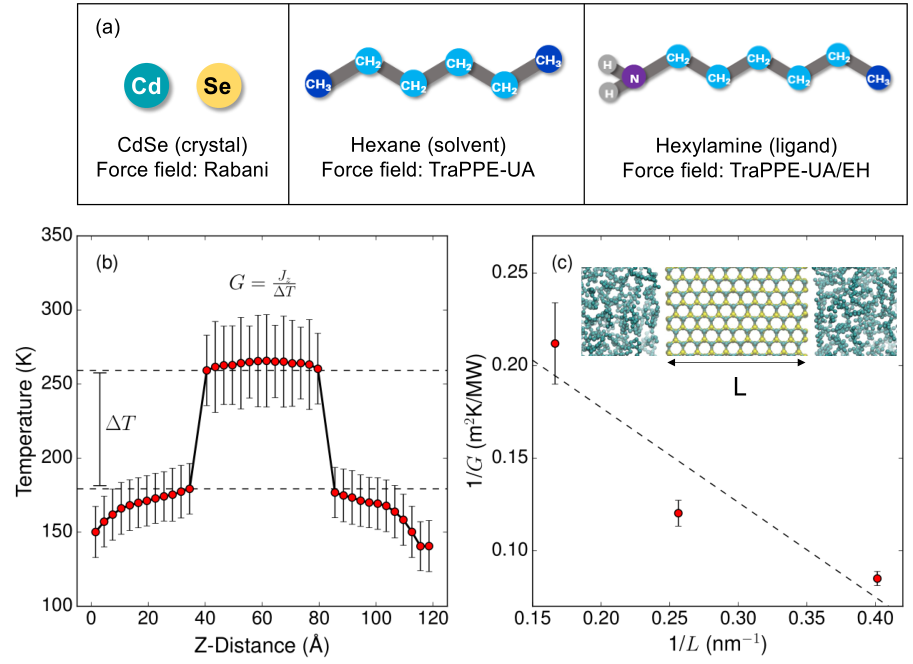
\includegraphics[width=\textwidth]{./Chapter4/rnemd2.png}
\caption[Details of RNEMD simulations of thermal transport at CdSe/hexane interfaces.]{ (a) Topologies of the molecules used in our simulations. The chemically distinct sites, given as colored spheres in the above diagram, are treated as united atoms. Amine headgroups are modeled with explicit hydrogen atoms \cite{doi:10.1021/jp0504827}. (b) Temperature profile along the kinetic energy exchange axis obtained for a system containing hexane and an unpassivated CdSe $11\bar{2}0$ slab. The discontinuities near 40 and 80 \r{A} represent the CdSe/hexane interface. The temperature drop at this interface, indicated by a dashed line in (a), is used to obtain the interfacial thermal conductance, $G$. Error bars are derived from temperature deviations in the bins along the production trajectory. (c) Inverse interfacial thermal conductance as a function of inverse slab length, $L$. As the length of the solvent region is also increased for larger simulations (fixed at $2L$), extrapolation to the y-intercept yields the interfacial thermal conductance for an infinitely thick slab of CdSe surrounded by an infinitely thick hexane bath. Inset: A snapshot from an MD trajectory used to produce this data. $L$ is indicated on the figure.}
\label{f:rnemd2}
\end{center}
\end{figure}

\begin{table}
\caption{RNEMD-Derived Interfacial Thermal Conductance Values for Four Surfaces of Wurtzite CdSe}
\centering
\begin{tabular}{l r}
\hline\hline
Surface & $G$ (MW/m$^2$/K) \\
\hline
$11\bar{2}0$ & 3.6 $\pm$ 0.9 \\
$10\bar{1}0$ & 1.7 $\pm$ 0.5 \\
$0001$ & 2.0 $\pm$ 0.6 \\
$000\bar{1}$ & 1.9 $\pm$ 0.6 \\
\hline
\end{tabular}
\label{table:rnemdT1}
\end{table}

Next, we probe the effects of surface passivation on the interfacial thermal conductance of the CdSe/hexane interface. Figure \ref{f:rnemd3} displays the temperature profile obtained for a completely passivated hexylamine-passivated $11\bar{2}0$ surface. Here, complete passivation is defined as having one hexylamine ligand for each surface atom, as described above. The temperature profile obtained here is more complicated owing to compositional heterogeneity and multiple interfaces. In this case, Eq. \ref{eq:rnemd3} is applied in the calculation of the interfacial thermal conductance. The interfacial thermal conductance values obtained for fully passivated hexylamine-passivated CdSe surfaces are summarized in Table \ref{table:rnemdT2}. To obtain average values of $G$, we performed four statistically independent RNEMD simulations of each surface. Statistical independence was ensured by generating initial velocity distributions from a different random seed for each replicated simulation. \par

\begin{figure}
\begin{center}
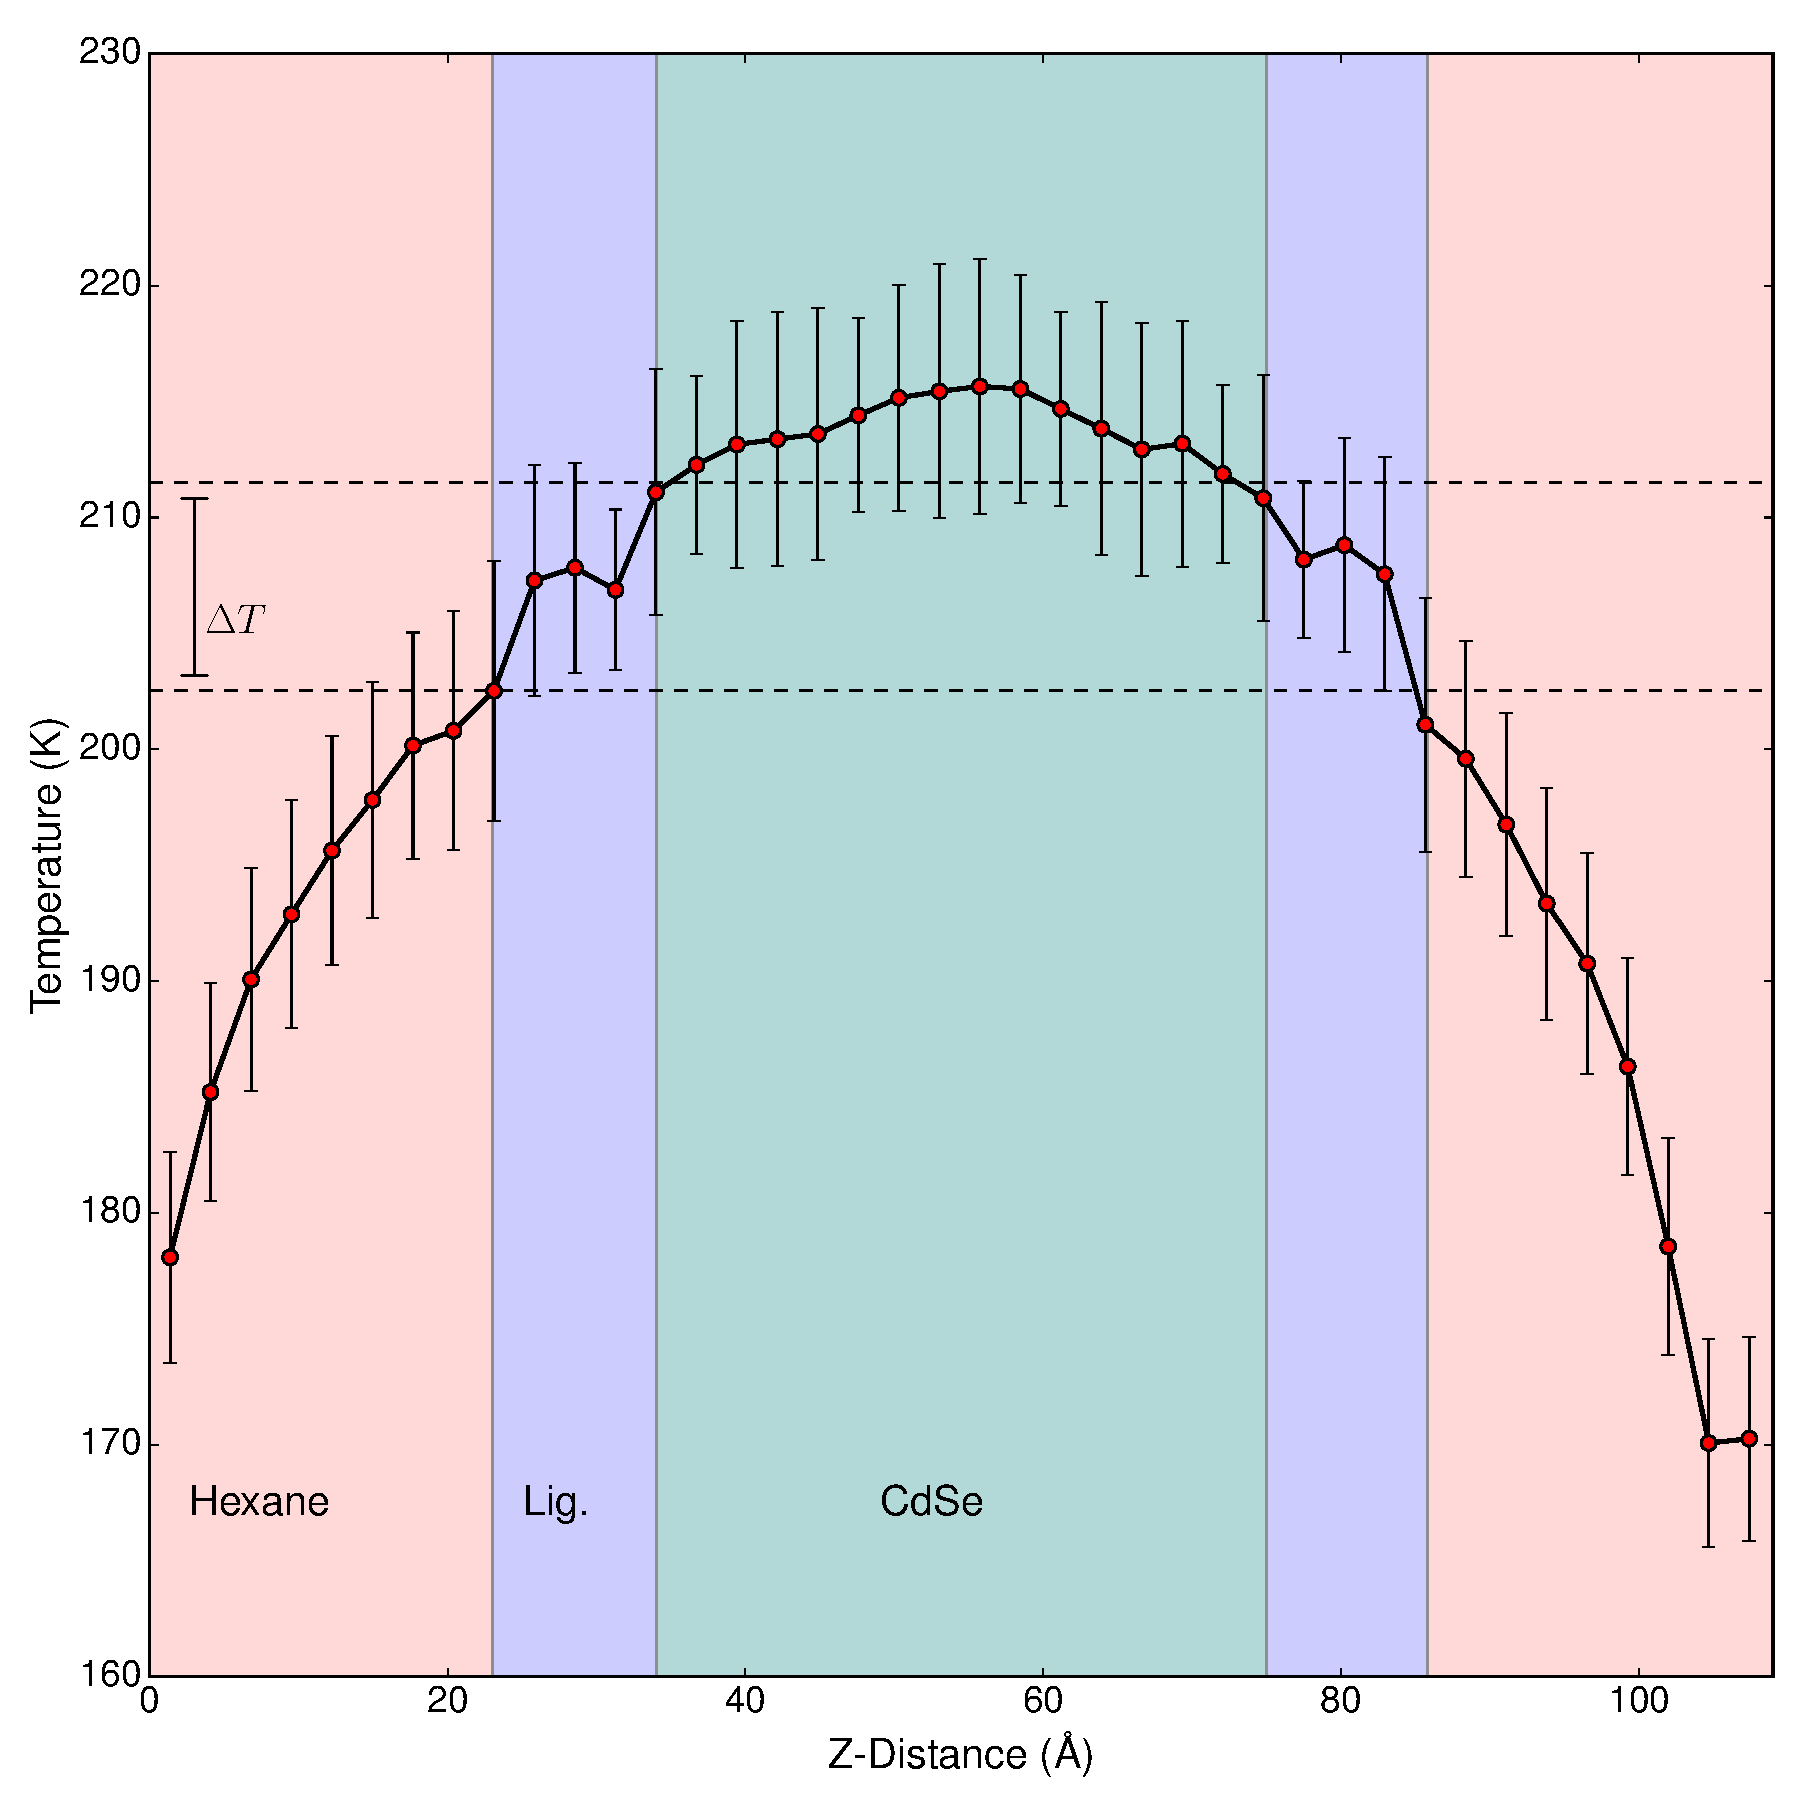
\includegraphics[width=\textwidth]{./Chapter4/rnemd3.pdf}
\caption[Temperature profile obtained from RNEMD simulation of CdSe/hexylamine/hexane interface.]{Temperature profile along the kinetic energy exchange axis obtained following a 3 ns RNEMD simulation of a system containing hexane (solvent) and a CdSe($11\bar{2}0$) slab passivated by hexylamine (ligand). The Z-coordinates corresponding to each region are labeled on the figure, with interfaces being designated by dashed lines. Error bars are derived from temperature deviations in the bins along the production trajectory.}
\label{f:rnemd3}
\end{center}
\end{figure}

\begin{table}
\caption{RNEMD-Derived Interfacial Thermal Conductance Values for Four Surfaces of Fully Passivated Wurtzite CdSe}
\centering
\begin{tabular}{l r}
\hline\hline
Surface & $G$ (MW/m$^2$/K) \\
\hline
$11\bar{2}0$ & 72 $\pm$ 12 \\
$10\bar{1}0$ & 80 $\pm$ 8 \\
$0001$ & 90 $\pm$ 7 \\
$000\bar{1}$ & 82 $\pm$ 11 \\
\hline
\end{tabular}
\label{table:rnemdT2}
\end{table}

As shown in Table 2, the presence of a passivating layer significantly increases the interfacial thermal conductance of a CdSe/hexane interface. This elevated thermal conductance can be understood in terms of improved vibrational overlap between CdSe and hexylamine as well as between hexane and hexylamine. Figure \ref{f:rnemd4}(a) displays the vibrational power spectrum of each distinct molecular component in the simulation cell (CdSe, hexylamine, hexane). The vibrational power spectrum is obtained by taking the Fourier transform of a velocity autocorrelation function obtained from 3 ns of simulation in an NVE ensemble subsequent to the pre-equilibration steps described above. This is shown in Equation \ref{eq:rnemd6}:
\begin{equation} \label{eq:rnemd6}
f(\omega) = \int^{+\infty}_{-\infty} \left\langle\vec{v}_A(t) \cdot \vec{v}_A(0)\right\rangle e^{-2\pi it\omega} dt
\end{equation}

\begin{figure}
\begin{center}
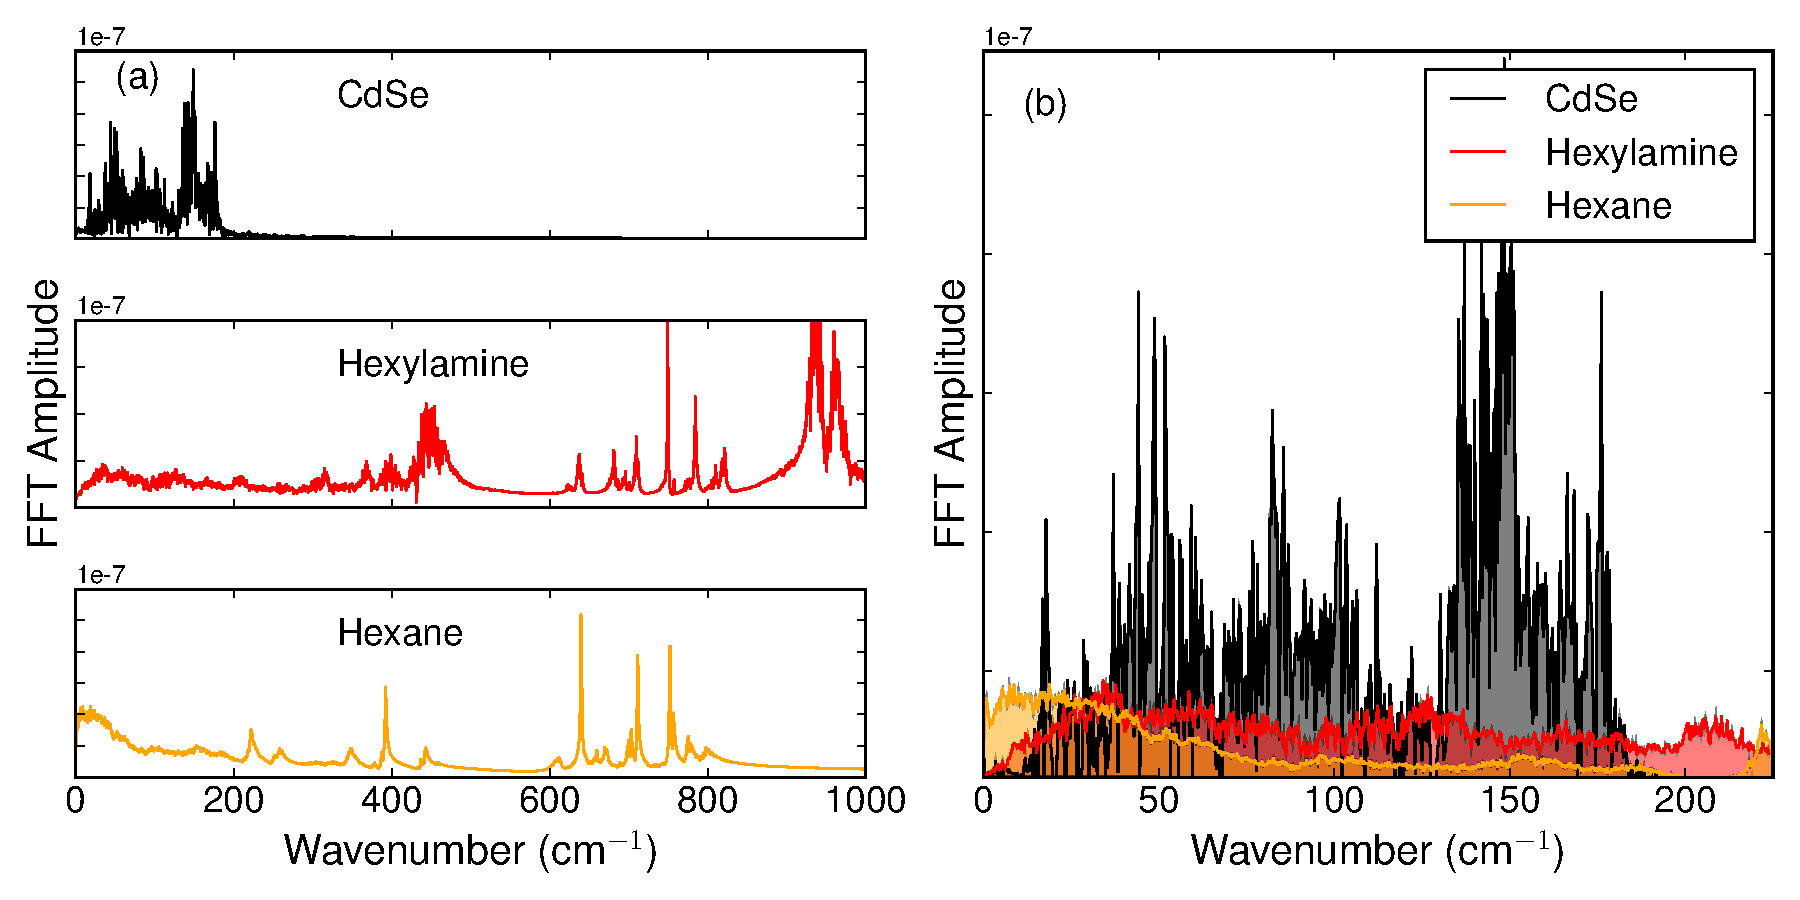
\includegraphics[width=\textwidth]{./Chapter4/rnemd4.pdf}
\caption[Vibrational power spectra for hexane, hexylamine, and CdSe.]{(a) Vibrational density of states at 200 K as obtained from Fourier transformation of the velocity autocorrelation function (eq 6) from an NVE simulation of a hexylamine-passivated, CdSe($11\bar{2}0$) surface surrounded by hexane. Each panel is labeled by molecular species. (b) Comparison of vibrational overlap at low frequencies. Hexylamine, shown in red, has a higher vibrational density of states than hexane (yellow) for most of this spectral region.}
\label{f:rnemd4}
\end{center}
\end{figure}

The hexylamine layer, shown in the middle of Figure \ref{f:rnemd4}(a), clearly exhibits greatly improved vibrational overlap with hexane, as these molecules are structurally and compositionally similar. Hexylamine also exhibits greater overall vibrational overlap with CdSe than hexane. This is emphasized in Figure \ref{f:rnemd4}(b), which focuses on the low frequency region containing the CdSe vibrational modes. \par

We also explore the dependence of interfacial thermal conductance on the extent of surface passivation. Figure \ref{f:rnemd5}(a) displays the interfacial thermal conductance as a function of ligand density on the surface, with each $G$ value (and its uncertainty) being the average (and standard deviation) of values obtained from four statistically independent RNEMD runs, as described above. Here, ligand density is defined as the number of hexylamine molecules in the simulation cell divided by the cross-sectional area of the CdSe slab. For the nonpolar $11\bar{2}0$ and $10\bar{1}0$ surfaces, $G$ increases roughly linearly with the extent of surface passivation. In contrast, the polar surfaces ($0001$ and $000\bar{1}$ show a nonmonotonic dependence of $G$ on the extent of surface passivation. Note, however, that the nonpolar $11\bar{2}0$ and $10\bar{1}0$ surfaces have a much lower atomic density and therefore do not support grafting densities as large as those supported by the polar surfaces. As indicated in \ref{f:rnemd5}(a), the highest ligand densities studied represent 100\% passivation of the surface, meaning that each surface site is interacting with a single passivating ligand. The polar CdSe surfaces have twice as many surface sites for a given cross-sectional area; this is demonstrated visually in Figure 5b, which highlights the number of surface sites for the $11\bar{2}0$, $10\bar{1}0$. and $0001$ surfaces. While no experimental estimate yet exists for the thermal conductance of CdSe/hexylamine/hexane interfaces, the $G$ values obtained here for maximal surface coverage are qualitatively similar to values experimentally measured for an oleate-passivated PbS nanocrystal array\cite{ong2013surface} and so are likely physically reasonable.

\begin{figure}
\begin{center}
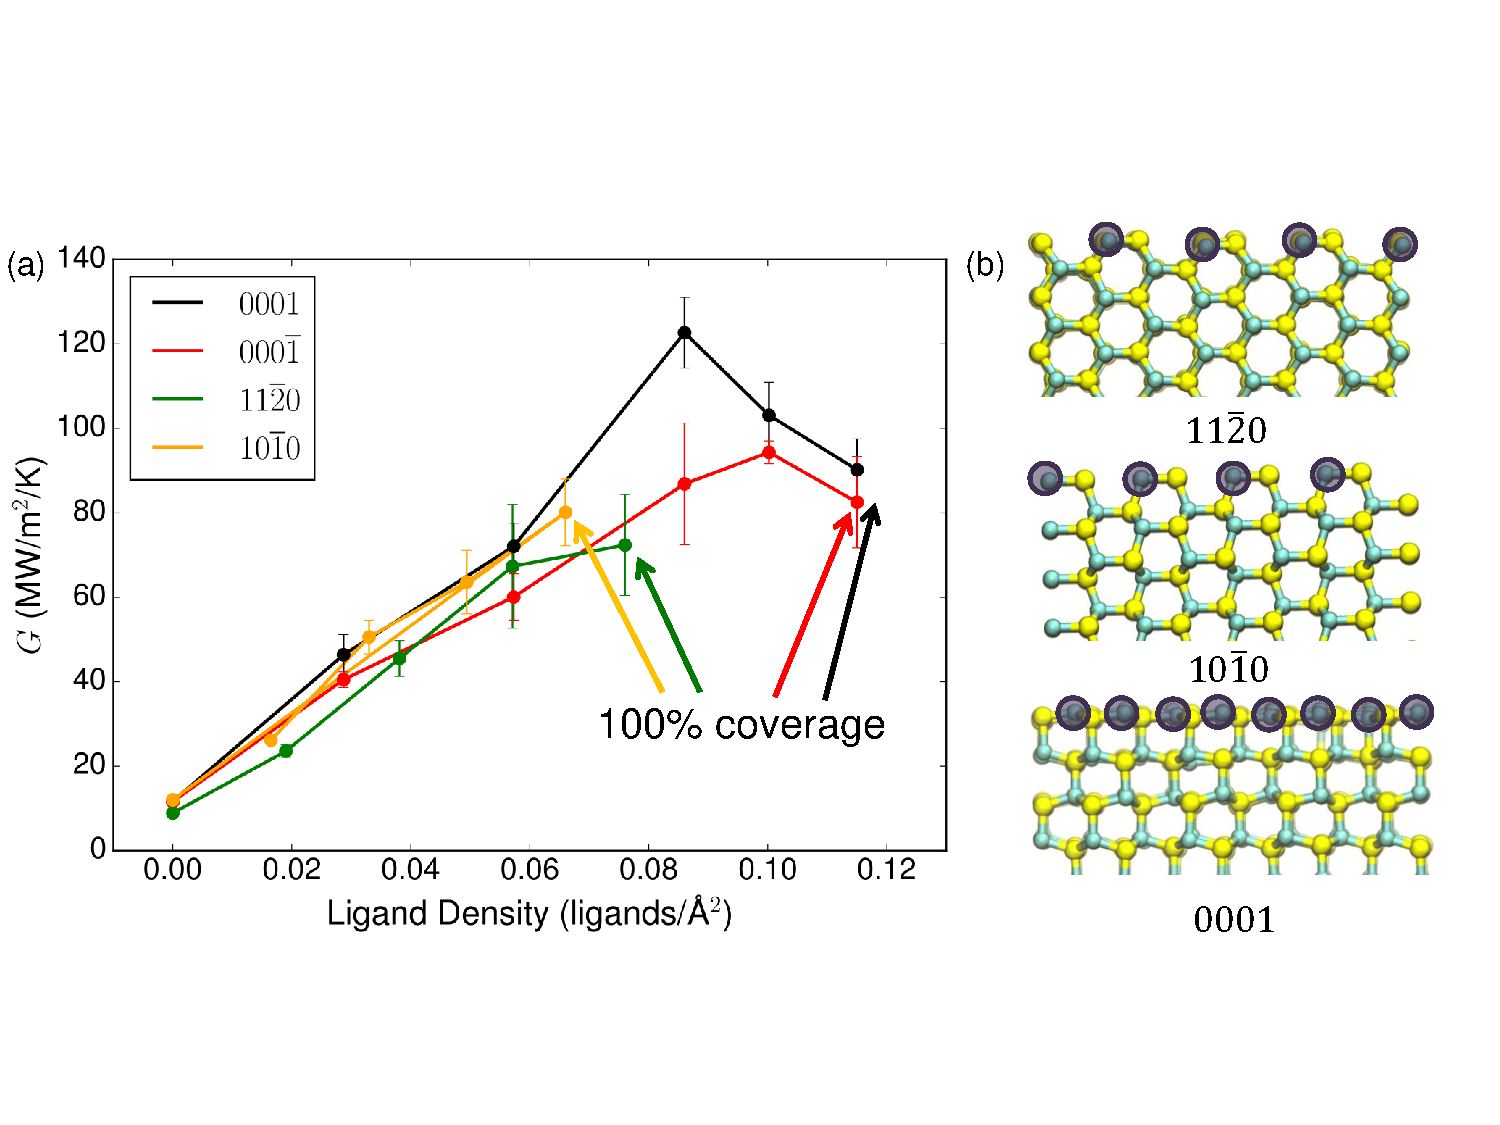
\includegraphics[width=\textwidth]{./Chapter4/rnemd5.pdf}
\caption[Dependence of interfacial thermal conductance on extent of surface passivation for a CdSe/hexylamine/hexane interface.]{(a) Vibrational density of states at 200 K as obtained from Fourier transformation of the velocity autocorrelation function (eq 6) from an NVE simulation of a hexylamine-passivated, CdSe($11\bar{2}0$) surface surrounded by hexane. Each panel is labeled by molecular species. (b) Comparison of vibrational overlap at low frequencies. Hexylamine, shown in red, has a higher vibrational density of states than hexane (yellow) for most of this spectral region.}
\label{f:rnemd5}
\end{center}
\end{figure}

The nonmonotonic dependence of $G$ on surface ligand density (Figure \ref{f:rnemd5}(a) can be understood as a balance of competing effects related to conduction, ordering, and excluded volume. First, surface ligands clearly facilitate heat conduction in the system via improved vibrational overlap (Figure \ref{f:rnemd4}). However, larger surface ligand densities also exclude solvent penetration into the ligand layer. Figure \ref{f:rnemd6} displays the time-averaged number density of both hexane (solvent) and hexylamine (ligand) along the kinetic energy exchange axis as obtained from analysis of RNEMD trajectories subsequent to the development of a stable temperature gradient. Density profiles for solvent and ligand resolved along the kinetic energy exchange axis can be found in Appendix E for all of the surfaces and ligand coverages examined in this Chapter. Higher ligand coverages clearly coincide with reduced solvent penetration into the same region; density profiles for each coverage can be found in Appendix E. Ligand and solvent molecules have a roughly equal number density at $\sim$35\% ligand coverage, which should maximize conduction effects, as every hexane molecule in the ligand layer, at least in principle, has a hexylamine partner available for coupling. This first-order analysis, however, ignores effects due to orientational ordering and solvent trapping in the ligand layer. \par

\begin{figure}
\begin{center}
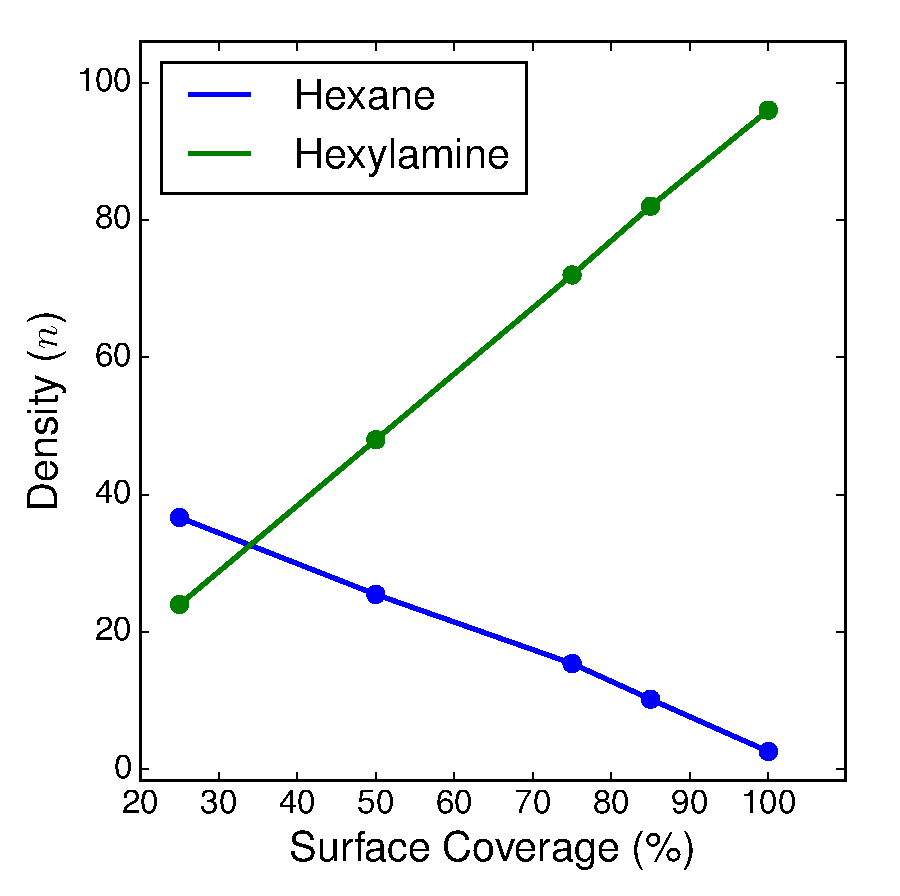
\includegraphics[width=0.5\textwidth]{./Chapter4/rnemd6.pdf}
\caption[Number density of hexane and hexylamine molecules in the hexylamine layer as a function of surface coverage.]{Integrated number density in the ligand region for ligand (hexylamine) and solvent (hexane) molecules as a function of surface coverage on a $0001$/$000\bar{1}$ CdSe slab. These curves intersect at roughly 35\% surface coverage.}
\label{f:rnemd6}
\end{center}
\end{figure}

While low ligand coverage permits greater solvent penetration into the ligand layer, these solvent molecules are less likely to be ordered in a fashion conducive to thermal energy transfer. As molecular alignment plays an important role in facilitating thermal energy transfer \cite{shen2010polyethylene}, the relative orientation of ligand molecules and solvent molecules in the ligand layer must be considered. Qualitatively, it is expected that higher ligand densities will force interpenetrating solvent molecules into alignment. This effect can be examined via diagonalization of an order parameter tensor given by Eq. \ref{eq:rnemd7}: \par
\begin{equation} \label{eq:rnemd7}
Q_{\alpha\beta} = \frac{1}{2N}\sum^N_{i = 1} \left(3\vec{e}_{i\alpha}\vec{e}_{i\beta} - \delta_{\alpha\beta}\right)
\end{equation}
In Eq. \ref{eq:rnemd7}, $\vec{e}_{i\alpha}$ is the $\alpha = x, y, z$ component of the unit vector $\vec{e}_i$, defined here as a vector along the terminal atoms of a given solvent or ligand molecule. The summation runs over all of the molecules being considered, with $N$ representing the total number of molecules of a particular type (solvent or ligand). The Kroenecker delta function is represented by $\delta_{\alpha\beta}$. The largest eigenvalue of $Q$ is traditionally used to obtain the orientational order parameter, while the eigenvector associated with that eigenvalue is the director axis, $\vec{d}(t)$. The director axis defines the average direction of molecular alignment at time $t$. The alignment of ligand molecules and entrapped solvent molecules can be quantified as the time-averaged dot product of the director axes of each respective molecule, as shown in Eq. \ref{eq:rnemd8}: 
\begin{equation} \label{eq:rnemd8}
\left\langle d \right\rangle = \left\langle \vec{d}_{hexylamine}(t) \cdot \vec{d}_{hexane}(t)\right\rangle
\end{equation}
This quantity ranges between 0 (hexane and hexylamine molecules aligned perpendicularly) and 1 (parallel alignment). This dot product is displayed as a function of ligand surface coverage in Figure \ref{f:rnemd7}(a) for a CdSe $0001$/$000\bar{1}$ surface. Generally $\left\langle d \right\rangle$ is larger for higher surface coverages, reflecting the formation of “pockets” which force interpenetrating solvent molecules into alignment \cite{doi:10.1021/jp312734f}. The anomalously low value of $\left\langle d \right\rangle$ for 100\% surface coverage reflects the near-complete exclusion of solvent from the ligand layer (Figure \ref{f:rnemd6}(e)). This alignment facilitates efficient thermal coupling, offsetting the decreased penetration of solvent into the ligand layer. \par

\begin{figure}
\begin{center}
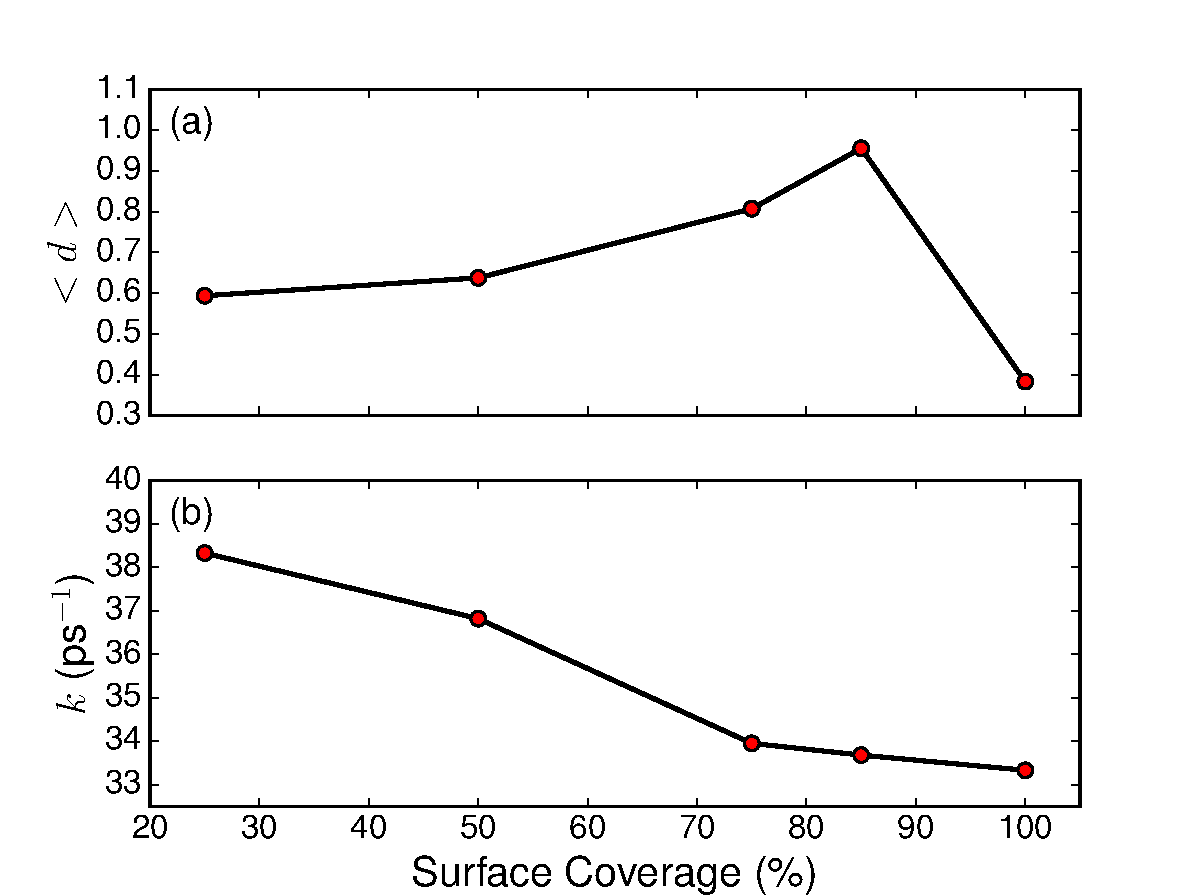
\includegraphics[width=0.75\textwidth]{./Chapter4/rnemd7.pdf}
\caption[Alignment and time-averaged residence time of solvent molecules in a passivating ligand layer on a CdSe surface.]{(a) Time-averaged dot product of the director axis for hexylamine molecules and hexane molecules present in the hexylamine layer, as defined in Eq. \ref{eq:rnemd8}, as a function of surface coverage for the $0001$/$000\bar{1}$ surfaces. (b) Solvent escape rate, $k$, as a function of surface coverage for the $0001$/$000\bar{1}$ CdSe surfaces.}
\label{f:rnemd7}
\end{center}
\end{figure}

In addition to the average density of solvent molecules in the ligand layer, the time scales of solvent movement into and out of the ligand layer are also of interest. To analyze these time scales, we utilize a survival correlation function which measures the residence time of a solvent molecule in the ligand layer. This function, $C(t)$, correlates the identity of all hexane molecules within the ligand layer at two times. If the solvent molecule is present at both times, the configuration contributes a 1, and contributes a 0 otherwise. A 0 contribution indicates that the solvent molecule has migrated back into the bulk liquid, and so a steep decay of $C(t)$ indicates a high turnover rate of solvent molecules in the ligand region. We define this solvent escape rate, $k$, for a simulation of duration $T$, according to Eq. \ref{eq:rnemd9}: 
\begin{equation} \label{eq:rnemd9}
k = \left(\int^T_0 C(t)dt)\right)^{-1}
\end{equation}
Figure \ref{f:rnemd7}(b) $k$ as a function of surface coverage. As surface ligand density increases, $k$ decreases, indicating that solvent molecules spend a longer time trapped in the ligand layer at high coverages. Depending on the time scale of heat transfer between the hexylamine ligands and hexane molecules in the ligand layer, the increased residence time of the solvent molecules at higher coverages my facilitate thermal transport by allowing the solvent molecules adequate time to thermalize with the ligands before returning to the bulk liquid. While $G$ does decrease for surface coverages yielding the lowest $k$ values, it is unlikely that the residence time of solvent molecules in the ligand layer is long enough to impede interfacial thermal conductance. Given the extremely small relative change in k ($\sim$2) over the 75-100\% surface coverage range, the decrease in $G$ is more likely a result of solvent exclusion (Figure \ref{f:rnemd6}), which eventually overwhelms positive contributions to interfacial thermal conductance due to orientational ordering and vibrational overlap. It is the interplay of these effects which ultimately yields the nonmonotonic dependence of $G$ on surface coverage for the polar CdSe surfaces (Figure \ref{f:rnemd5}(a)).

\subsection{Conclusion}
Our results highlight the important role played by surface chemistry and crystal structure in mediating thermal transport across chemically passivated semiconductor interfaces. Generally, passivation of a CdSe surface with hexylamine increases the thermal conductance of the interface by more than 1 order of magnitude. Furthermore, we find that while $G$ increases with increasing surface coverage at lower ligand-grafting densities, $G$ decreases at the highest grafting densities. \par

The nonmonotonic dependence of $G$ on surface coverage is a manifestation of several competing phenomena. Hexylamine (the passivating ligand) exhibits improved vibrational overlap with both CdSe and hexane (the solvent). The presence of hexylamine thus facilitates efficient thermal coupling in the system. However, as ligand grafting on the surface becomes increasingly dense, exclusion of solvent molecules from the ligand layer occurs. At the same time, higher ligand coverage tends to force into alignment any solvent molecules which do manage to penetrate into the ligand layer, yielding more efficient vibrational coupling of these molecules. Higher coverages also result in decreased solvent escape rates, though these decreases are unlikely to play a dominant role in determining $G$. Taken in aggregate, these effects produce maximal interfacial thermal conductance at ligand-grafting density values in the range of 0.08-0.1 ligands/\r{A}$^2$. These grafting density values represent a fractional coverage that varies for a particular facet. For the nonpolar surfaces ($10\bar{1}0$, and $11\bar{2}0$), a ligand-grafting density of 0.08 represents a full monolayer (all binding sites occupied), while the same grafting density represents roughly 75\% of a monolayer for the polar surfaces ($0001$ and $000\bar{1}$). The ligand-grafting density corresponding to a full monolayer (100\% coverage) for each surface is indicated in Figure \ref{f:rnemd5}(a). \par

While the interfacial thermal conductance of bare CdSe surfaces was found to be similar for each of the surfaces studied, crystal structure nevertheless plays an extremely important role, as the number of available binding sites on each surface ultimately determines the limit of ligand-grafting density. For example, for the wurtzite crystal structure, passivated nonpolar surfaces exhibit much lower interfacial thermal conductance than passivated polar surfaces owing to fewer binding sites per unit area of the nonpolar surface. As synthetic methods for semiconductor nanocrystals have become increasingly sophisticated, particularly for metal chalcogenide nanocrystals, chemical control of the surface areas of each facet has become a possibility. Our results therefore have interesting implications for the synthetic manipulation of interfacial thermal conductance in this technologically important material class. \par

The specific case of a crystalline CdSe semiconductor material was examined in this work, but the phenomena identified are general. The dependence of ligand-grafting density (and, thus, interfacial thermal conductance) on the particular exposed surface is a previously unreported phenomenon; prior studies examining gold surfaces find that ligand-grafting density is primarily determined by the steric behavior of the ligands. This effect likely stems from the fact that CdSe is a binary compound and only half of the exposed atoms on a nonpolar surface will interact strongly with ligands, resulting in lower overall grafting density for these surfaces. The hexagonal lattice and different structural parameters of CdSe as compared to Au may also play a role. Regardless, our results highlight for the first time the possibility of atomic structure on the exposed crystal surface being the primary factor in determining the interfacial thermal conductance of chemically passivated interfaces. In the limit that interfacial thermal conductivity dictates the overall thermal transport rate involving a semiconductor, variation in the surface termination and exposed surface area offers a route to anisotropic transport that can aid thermoelectric efficiencies or improve heat dissipation from LEDs, lasers, and solar cells.
